\documentclass[a4paper, 12pt]{report}
\usepackage[T1]{fontenc}
\usepackage[utf8]{inputenc}
\usepackage[english]{babel}
\usepackage{mathtools}
\usepackage{amsfonts}
\usepackage{amsmath}
\usepackage{mathrsfs}
\usepackage{enumitem}
\usepackage{booktabs}
\usepackage{array}
% Avoid paragraph indent
\setlength{\parindent}{0pt}
% Useful floor and ceiling functions
\DeclarePairedDelimiter{\floor}{\lfloor}{\rfloor}
\DeclarePairedDelimiter{\ceil}{\lceil}{\rceil}
% Modified margins
\usepackage[margin=2cm]{geometry}
% This avoids hypenation
\hyphenpenalty=10000
\usepackage{tikz}
\usetikzlibrary{arrows,calc,positioning,shadows,shapes}
\usepackage{graphicx}
\usepackage{subfig}
\captionsetup[figure]{labelfont={bf},name={Figure},labelsep=period}
\captionsetup[table]{labelfont={bf},name={Table},labelsep=period}

\usepackage{float}


\begin{document}
	
\title{Digital Communications and Laboratory \\ Second Homework}
\author{Faccin Dario, Santi Giovanni}
\date{}
\maketitle

\section*{Problem 1}

\section*{Problem 2}

A flat fading channel with only one top $h_0(nT_c)$ was studied, assuming a \textit{Rice factor} of k=2 dB and normalized $M_{h_0}$. Moreover, a classical \textit{Doppler Spectrum} with $f_d T_c=40\cdot10^{-5}$ was considered. The schematic model to generate the coefficient $h_0$ of the channel is given in Figure \ref{Model_2}.

\begin{figure}[H]
	\centering
	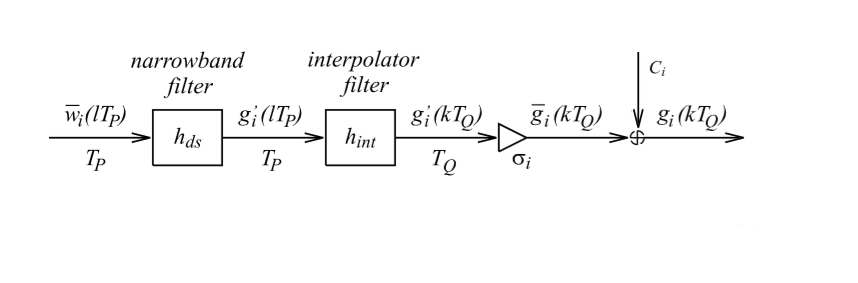
\includegraphics[width=14cm]{images/Model_2}
	\caption{Model to generate the coefficient $h_0$ of the time-varying channel.}\label{Model_2} 
\end{figure}

The Doppler Spectrum can be generated using a filter $h_{ds}$ such that $|\mathcal{H}_{ds}(f)|^2 = D(f)$.\\
In Table \ref{iircoeffs} are shown the coefficients used for such filter \cite{nevio<3}:

\begin{table}[H]
	\centering
	\begin{tabular}{c c c c}
		\toprule
		\textbf{$H_{ds}(z) = B(z)/A(z)$} & $f_dT_p=0.1$ &  &     \\
		\midrule
		$ \{a_n\} $ ,& $n=0, \dots, 11$:  & & \\
		1 & -4.4153 & 8.6283 & -9.4592   \\
	    6.1051 & -1.3542 & -3.3622 & 7.2390 \\
	    -7.9361 & 5.1221 & -1.8401 & 2.8706e-1 \\
	    \midrule
	    $ \{b_n\} $ ,& $n=0, \dots, 21$:  & & \\
	    1.3651e-4 & 8.1905e-4 & 2.0476e-3 & 2.7302e-3 \\
	    2.0476e-3 & 9.0939e-4 & 6.7852e-4 & 1.3550e-3 \\
	    1.8076e-3 & 1.3550e-3 & 5.3726e-4 & 6.1818e-5 \\
	    -7.1294e-5 & -9.5058e-5 & -7.1294e-5 & -2.5505e-5 \\
	    1.3321e-5 & 4.5186e-5 & 6.0248e-5 & 4.5186e-5 \\
	    1.8074e-5  & 3.0124e-6  & & \\
	    \bottomrule			
	\end{tabular}
	\caption{Coefficients for the IIR filter}
	\label{iircoeffs}
\end{table}


The graphical representation of the impulse response of the IIR filter and the Doppler Spectrum is shown in Fig. \ref{DS}. 
To obtain $h_0$, following the scheme of Fig. \ref{Model_2}, the noise component $w\sim \mathcal{CN}(0,1)$ is filtered with the IIR filter previously described. Note that the frequency response of this filter is $\mathcal{H}_{ds}(f)=\sqrt{\mathcal{D}(f)}$ while the PSD of the noise is constant and equal to 1. For this reason, the equivalent impulse response of this part is equal to $\mathcal{D}(f)=1\cdot |\mathcal{H}_{ds}|^2$ which is actually the Doppler spectrum. \\
The output of the filter is affected by a transient, which we avoided by considering only values after $5N_{eq}T_p$, where $N_{eq} = \left\lceil -\frac{1}{\ln(|p|)} \right\rceil$ is the equivalent time constant, and $p$ is the pole with the highest magnitude. Then, after scaling the coefficient such that $M_{h_0}/\sqrt{E_{h_{ds}}}=1$, the signal is filtered with an interpolation filter of factor $1/T_Q = T_p/T_c=250$. \\
The interpolator output signal is then multiplied by a constant $\sigma_0 = \sqrt{M_d}$ to impose the desired power delay profile, and finally added up with another constant, $C$, which included the deterministic component according to \cite{nevio<3}, Page 307.

\begin{figure}[H]
	\centering
	\subfloat{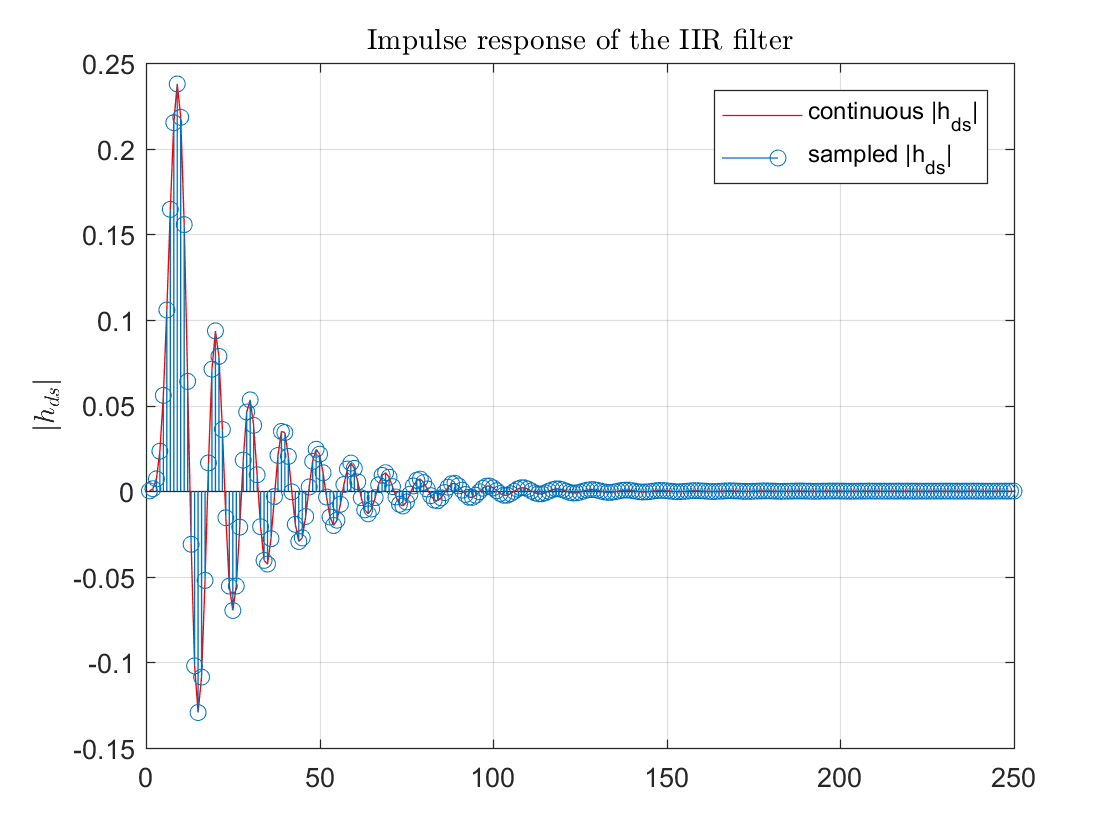
\includegraphics[width=7.5cm]{images/h_d}}
	\subfloat{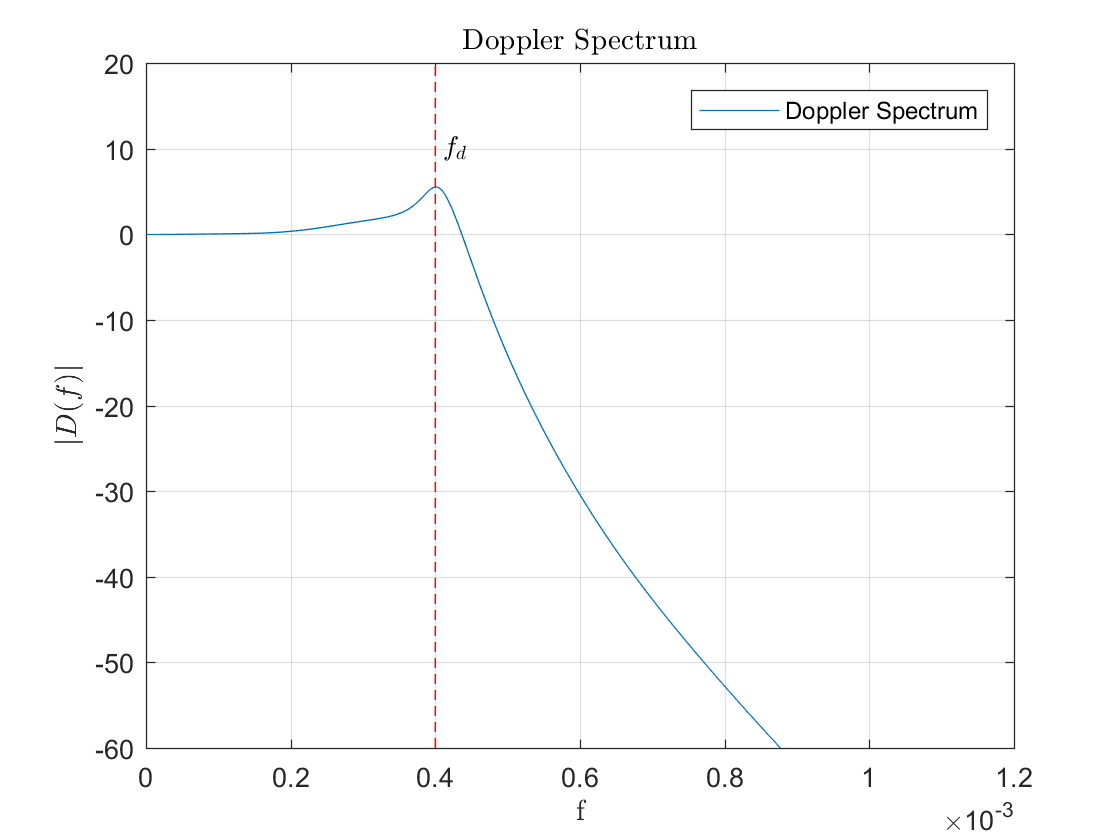
\includegraphics[width=7.5cm]{images/D}}
	\caption{Impulse response of the IIR filter and Doppler Spectrum}
	\label{DS}
\end{figure}

\subsection*{Estimate of $\mathbf{\frac{|h_0|}{\sqrt{M_{|h_0|}}}}$}ù




\begin{thebibliography}{15}
	\bibitem{nevio<3}
	Nevio Benvenuto, Giovanni Cherubini,
	\textit{Algorithms for Communication Systems and their Applications}. 
	Wiley, 2002.
\end{thebibliography}

\end{document}